\section{Demonstration Details}
\label{sec:dd}
 In this demonstration, we will use \GSQL\ to quantify the causal effect of
 different weather conditions on flight departure delay. 
    \paragraph{\bf Data:} The analysis we be conducted on a spatio-temporal join of the following datasets:
 \begin{itemize}
   \item {\it Flight dataset (105M entries)}: collected by the US
Department of Transportation (U.S. DOT).\footnote{\url{http://www.transtats.bts.gov/}} It contains
records of more than 90\% of US domestic flights of major airlines
from 1988 to the present. It includes attributes such as FlightDate, OriginAirportID (origin airport ID), CarrierID, CRSDepTime (scheduled departure time), and DepDelay (departure delay).
   \item {\it Weather dataset (40M entries):} historical weather data for relevant flight gathered using the weather underground API.\footnote{\url{https://www.wunderground.com}} It includes Code (Airport ID),
Date, Time,  Visim (visibility in km),
  Tempm (Temperature in C$^{\circ}$)
  Wspdm (wind speed kph), Pressurem (Pressure in mBar), Precipm  (Precipitation in mm), Snow (binary), Thunder (binary).
 \end{itemize}


 



\begin{figure*}
\begin{subfigure}{0.50\linewidth}
\centering
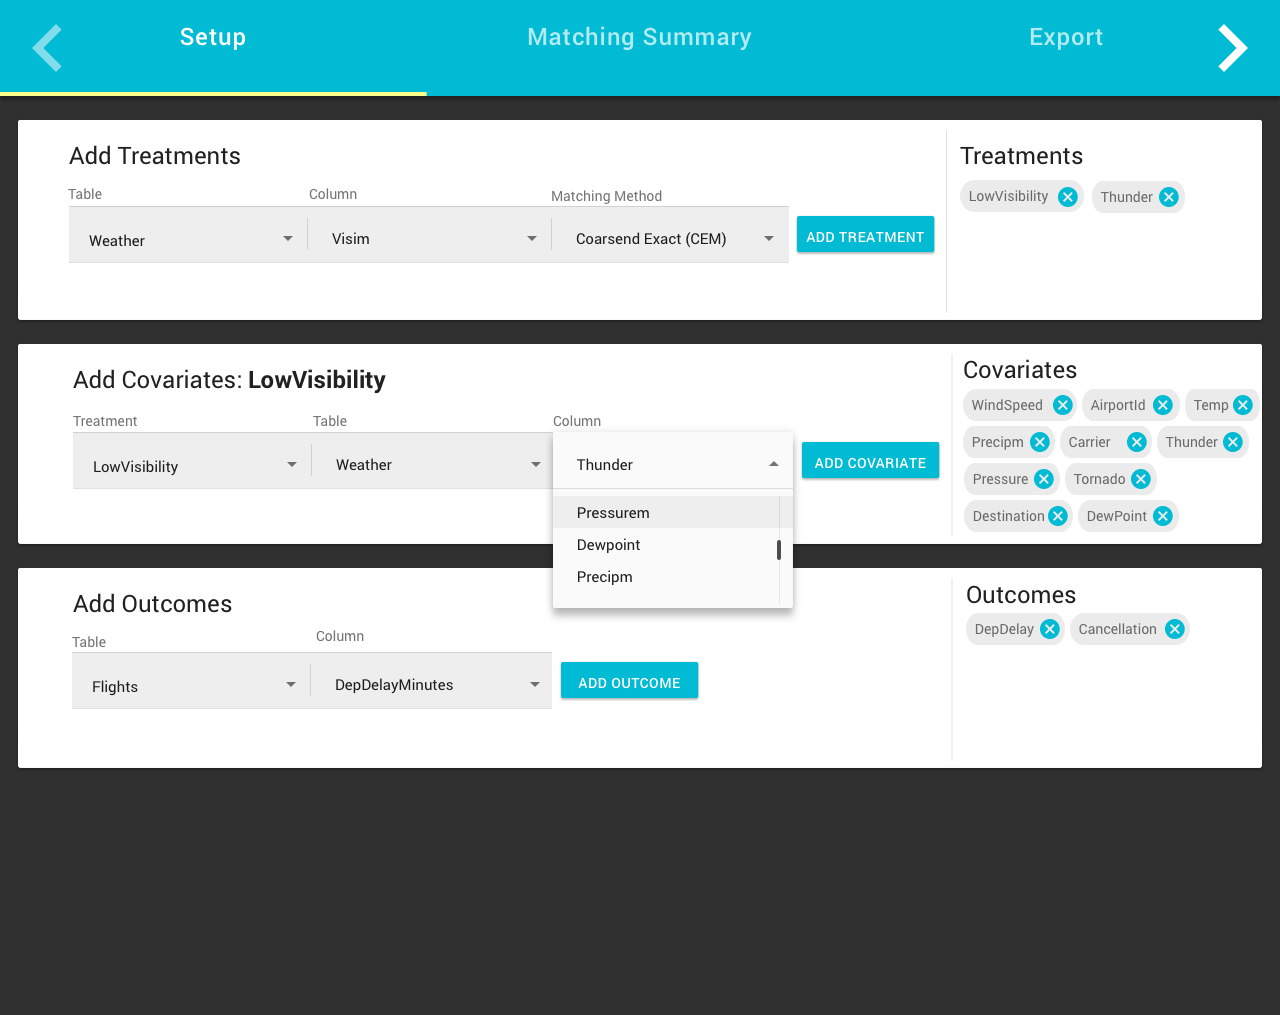
\includegraphics[scale=0.13]{Figures/Setup.png}
\label{sfig:testc}
\end{subfigure}\hfill
\begin{subfigure}{0.47\linewidth}
\centering
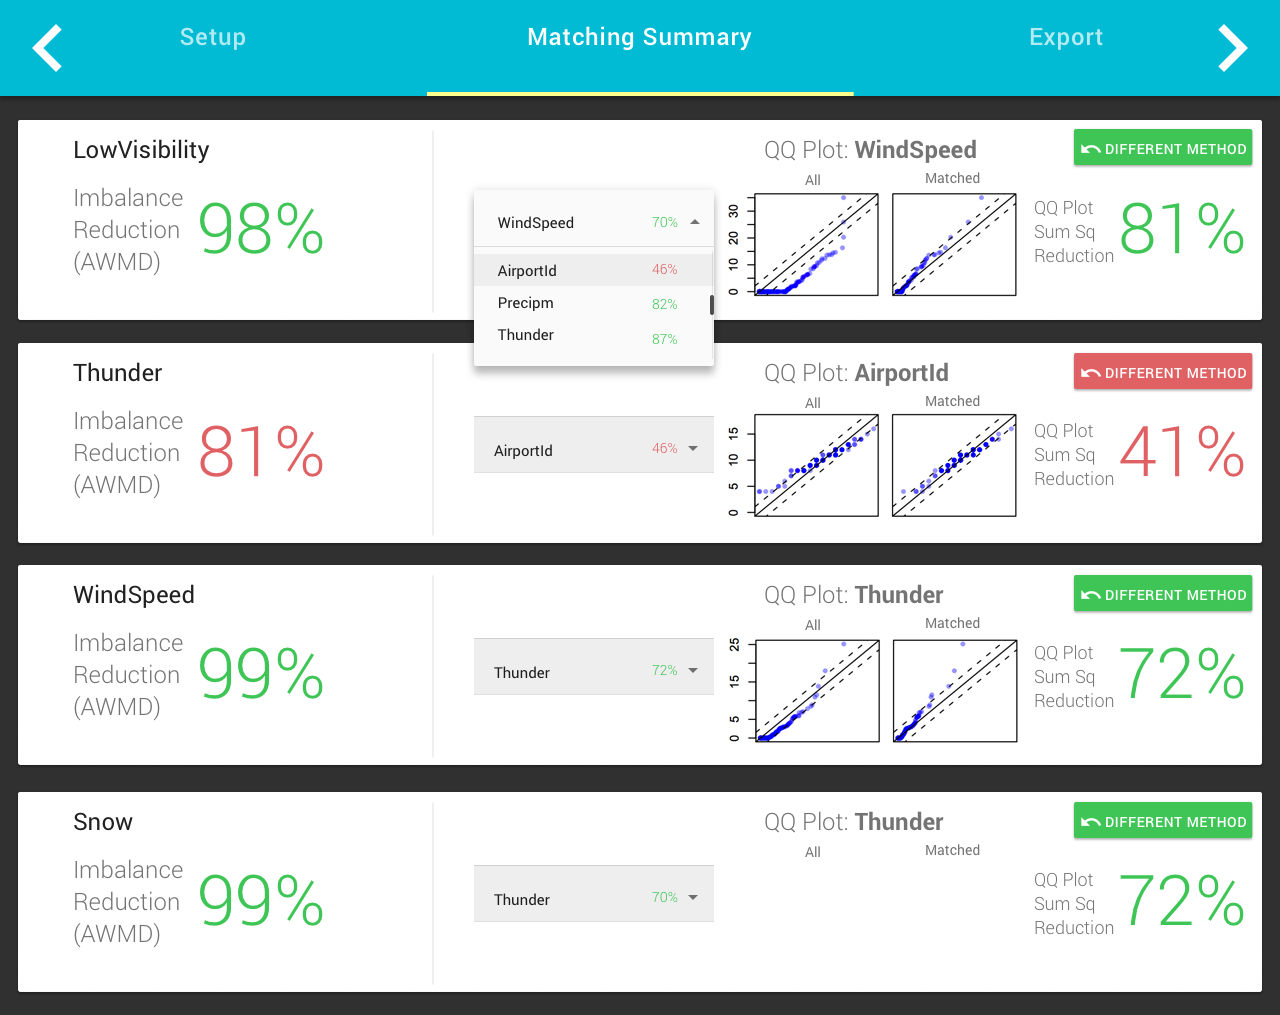
\includegraphics[scale=0.13]{Figures/Matching-Summary.png}
\label{sfig:testd}
\end{subfigure}\hfill
\caption{Demonstration Screenshot described in Section \ref{sec:dd}}
\label{fig:eteresult}
\end{figure*}








 
 \ignore{
 The analysis will be conducted on
 {\em flight data (105M eateries)}-collected by the US Department of Transportation (U.S. DOT)- and  {\em weather dataset} (10M eateries)-gathered using the weather underground
API. }

 \ignore{
 The {\em flight dataset} we use was collected by the US Department of Transportation (U.S. DOT) \cite{flightdata}. It contains
records of more than 90\% of US domestic flights of major airlines
from 1988 to the present. The {\em weather dataset} was gathered using the weather underground
API \cite{Weatherdata}.  \ignore{Its attributes are also presented in Table
\ref{tab:attlist}. In addition, we pre-computed two other attributes
AiportTraffic and CarrierTraffic. The former is the total number of
flights occur in the origin airport of a flight one hour prior to the
flight departure time, the latter is the same quantity restricted to
the flights from the same carrier.  We managed to acquire and clean
35M weather observations between 2000 and 2015.} These datasets are
integrated by a spatio-temporal join.}



\ignore{

        \caption{Weather dataset}
    \end{subtable}
 \vspace{-0.1cm}   \caption{\bf{List of attributes from the flight(a) and weather(b)  datasets that are relevant to our analysis.}}
\label{tab:attlist}
\end{table}
}



\begin{figure}
  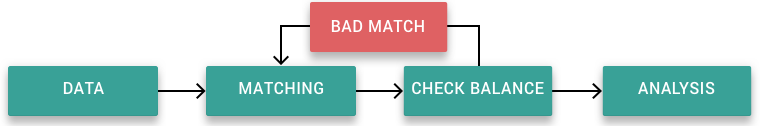
\includegraphics[scale=0.25]{Figures/Matching-Flowchart.png}
\caption{Causal Analysis Workflow}
\label{fig:flowchart}
\vspace{-0.3cm}
\end{figure}






\ignore{
\begin{example} \em \delay (cont.) \ \em   Suppose we want to explore the effect of the low-pressure (treatment) on flight departure delays (outcome).  The direct comparison of
delay between flights that happen during low-pressure (treated groups) and opposite (control group) is misleading.  It is known that high pressure is generally associated with clear weather,    while low-pressure is associated with unsettled weather, e.g.,
    cloudy, rainy, or snowy weather\ignore{\cite{weba2,barometricpressureheadache:article}}. Thus, as shown in Figure \ref{fig:cv}, factors such as thunder, snow, visibility confound pressure and delay. Therefore, conducting any sort of predictive analysis identifies
    low-pressure as a predictor for flight delays.
  However, low-pressure does not have any causal impact on departure delay
    (low-pressure only requires longer takeoff distance) \cite{FAA08}. In this demonstration, by conducting a careful causal analysis using \GSQL, we show that low-pressure is only a correlated attribute with flight delays and has no significant causal impact on flight delay.

    \ignore{By performing a careful casual analysis
    \GSQL\ found that other attributes such as thunder, low-visibility, high-wind-speed and
    snow have the largest causal effect on flight delays (see Sec. \ref{sec:endtoend});
  this is confirmed by the results reported by the FAA.}
\end{example}
}

% They defined a very simple model, where we
% want to conclude \dan{Lise: what's your comment here?}  if one
% variable, called ``treatment'' causes one particular output variable,
% called ``effect'', and have developed a rich set of techniques for
% that purpose.  The end goal of their analysis is to establish the
% average causal-treatment effect.  More recently, in the AI literature
% Pearl~\cite{pearl2010introduction,PearlBook2000} has extended this
% simple model by introducing {\em causal networks}, and developing a
% logical framework for reasoning about causality.  Their aim is to
% enable complex inference in a network of causal associations.  While
% the ultimate goal is the same, to check whether a particular input
% causes a particular outcome, the methods deployed are different from
% those in statistics.

\vspace{-0.1cm}

\ignore{
This paper makes the following specific contributions: we describe a
suite of techniques for expressing the existing advanced methods for
causal inference from observational data in SQL that run at scale
within a database engine (Section \ref{sec:BasicTechniques}). Note
that we do not claim any contribution the existing methods; we
introduce several optimization techniques that significantly speedup
causal inference, both in the online and offline setting (Section
\ref{sec:OptimizationTechniques}); we validate our system
experimentally, using real data from the U.S. DOT and Weather
Underground \cite{flightdata,Weatherdata}
}

\ignore{
Roughly speaking, in order to draw a valid causal conclusion one needs to control for the
confounding influences that affect both the treatment and outcome. Popular methods for
performing this task in statistics and social science are {\em subclassification and matching} \cite{Rubin1983b,IacKinPor09,rosenbaum1984reducing}.
The key goal of matching is to prune data so that
the remaining data have better balance between the treated and control groups meaning that the empirical distributions of the confounding variables (a.k.a, covariates) in the groups are more similar.  Since there is no generic metric to compare
two distributions a rule of thumb is to evaluate different matching methods and balance measures  until a well-balance matched subset with
a reasonable size obtained \cite{IacKinPor09} (See Figure \ref{fig:flowchart}).
}



\ignore{
\begin{enumerate}
\item {\it Selecting a causal hypothesis:}
  the attendee selects a causal hypothesis to test by specifying a treatment (potential cause)
  and an outcome (potential effect) (cf, Example \ref{sfig:testaa}).
\item {\it Matching method:} The user select a matching method to
\item Enable attendees to drill into the details of how we generate these
results (i.e.\, the different steps of the pipeline).
\item Show what happens for different configurations of the Viska system:
e.g.\, different parameters to graph-generation algorithms, different bucketing
strategies, \ldots
\end{enumerate}
}



  \paragraph{\bf Causal Questions:} demonstration starts by creating a set of causal questions regarding the effect of different weather attributes on flight delay by
    \begin{enumerate}
      \item specifying DepDelay as our outcome of interest (potential effect) as shown in Figure \ref{fig:eteresult}(a).
      \item specifying a set of binary treatments (potential causes) that might affect DepDelay. In particular the following binary treatments will be created: LowVisibility (1 if Visim$<1$; 0 if Visim$>5$); \ HeavySnow (1 iff Precipm$>0.3$ and Snow$=1$); \ WindSpeed (1 if Wspdm$>40$; 0 if Wspdm$<20$); \  Thunder; \ LowPressure (1 if Pressurem$<009.14$; 0 if Pressurem$>1022.69$).
      \ignore{
      As shown in Figure \ref{fig:eteresult}(b) Clicking on the {\it ADD TREATMENT}, {\it ADD COVARIATE}, and {\it ADD OUTCOME} buttons will trigger a dialog allowing
  further customization on the discretization and matching methods.
These dialogs will also allow the user to incorporate other columns (e.g. snow is defined as $iff Precipm> 0.3 and
Tempm< 0$) and input SQL for custom discretization methods.}
      
      \item specifying a subset of data that is relevant to the analysis.  We select five US airports  with hight rate of weather-related delay namely, San Francisco (SFO) , John F. Kennedy (JFK), Newark Liberty (EWR), George Bush (IAH), and LaGuardia Airport (LGA).
\end{enumerate}


 \paragraph{ \bf Computing ATE}: For each treatment, say LowPressure, \GSQL\ computes {\em average treatment effect (ATE)} as $$E[\text{Depdelay}|\text{LowPressure}=1] - E[\text{Depdelay}|\text{LowPressure}=0],$$
  where, E[\text{Depdelay}|\text{LowPressure}=$x$], $x=(0,1)$ is computed by taking the emetical average of  Depdelay where LowPressure is  $x$. ATE is a measures to compare DepDelay in the {\em treated group}, i.e., those subjects (flights) with LowPressure=1, with the {\em control group}, those with LowPressure=0.
 For example, for the treatment of LowPressure we obtain a relatively large number. This suggests  LowPressuret affects DepDelay. However, it is known that
  LowPressure does not have any causal impact on DepDelay (LowPressure only requires longer takeoff distance) \cite{FAA08}. This raises the question that that where is this difference coming from?

 \paragraph{\bf Confounding variables:} We address the question, by demonstrating that the comparison of DepDelay between the treated and control groups is misleading due to the exitance of the so-called {\em  confounding influence} of other variables such as visibility, snow and Thunder.  We show that, LowPressure is highly associated with unsettled weather conditions such as LowVisbility. For instance the average of LowVisbility in the treated group is much less than
  the opposite group. Thus, its is unclear that the observed DepDelay difference between the groups is causes by LowPressure or LowVisbility. This scenario, as shown graphically in Figure \ref{fig:cv}, demonstrates that in the presence of {\em confounding variable} (a.k., {\em covariates}) the treated and control groups are very different. Thus, comparing the groups without accounting for the confounding variables could be misleading.


 \paragraph{\bf Controlling confounding influence:}
In this step we use \GSQL\ to apply state-of-the art methods for controlling confounding influences.
In particular, we use the popular methods developed in social science and statistic namely,  {\em subclassification} and {\it propensity score matching} \cite{Rubin1983b,IacKinPor09,rosenbaum1984reducing}. Throughout the demonstration we will refer to them as matching methods.
The key goal of matching is to prune data so that
the remaining data ({\em matched data}) have better balance between the treated and control groups meaning that the empirical distributions of the confounding variables in the groups  similar. 
Once the two groups become similar, any observed different of outcome between the two group can attributed to the treatment. Now,
     \begin{enumerate}
      \item for each treatment, we select a set of covariates deemed to confound with the the DepDelay (Figure \ref{fig:eteresult}(d)).
      \item we select a matching method and adjust its tuning parameters (Figure \ref{fig:eteresult}(e)).
\end{enumerate}

\paragraph{\bf Checking Balance:}  In this step we check wether the matching process was successfully improved covariates balance by
    \begin{enumerate}
      \item comparing the distribution for each covariate between the treated and control group on matched data. For this task, \GSQL\  provides numerical summaries such as the mean Diff. (difference in means), and summaries based on quantile quantile plots and multivariate histograms \ref{fig:eteresult}(d).

      \item We perform different matching methods with difference turning parameter to show these methods trade of balance and size of matched data to demonstrate the advantage and disadvantage of different methods.
       \end{enumerate}
      The main objective of this step is to demonstrate the typical worlkflow of causal inference from observational data. As shown in Figure \ref{fig:flowchart} it consists of the iterative process of matching and balance checking. This highlights the demand for tools such as \GSQL\, which perform matching at scale.

     \paragraph{\bf Answer to the causal questions:} In this step of the demonstration we answer the causal question created at the very fist step of the demonstration. 
       \begin{enumerate}
       \item for each treatment we compute ATE on the well-balanced matched subset of the data.
      \item we evaluate the statistical significance of the obtained result by performing an statistical test, e.g., Chi-square, test.
    \item we report major causes of flight delay at the airport under study.
    \item    we show that the results are in accordance with 
FAA, \footnote{\url{https://www.faa.gov/}} which reported the following major weather-related
causes:
snowstorms,thunderstorm and wind at EWR; thunderstorm and fog at IAH;
snowstorms and visibility at JFK; snowstorms at LGA; fog and low
clouds at SFO;
 
        \end{enumerate}



\paragraph{\bf Scalability:} In the final step of the demonstration we compare the scalability
of \GSQL\ with the other statistical softwares.  


